\section{Signal Start Detection}
\label{sec:03_signalStartDetection}

As mentioned in \ref{sec:02_signalStartDetection}, the detection of the
signal start is crucial for the localization.
The implementation of the different methods will be presented coupled with
an examination of real measurement data.
To reduce undesirable effects and demonstrate the simplest form, a sinusoidal
signal of $3000\si{Hz}$ with a sample rate of $44100\si{Hz}$. For this
data, the sound source was placed $2\si{m}$ in front of the robot.\\
In order to find the time point where the signal starts, information about
smaller fractions are required.
So, the original $44100$ samples that were buffered by the
\change[]{correct font and wording}
"WhistleLocalization" module are divided into several overlapping
frames with size $256$. The computational effort raises with smaller frame size,
but delivers a higher precision in return.
To compute the energy and entropy, the frames are transformed into
frequency domain with the \ac{FFT}.
The \ac{ZCR} does not require such a transformation.
\missing[]{final start index by combination of these 3 methods}
For better visualization, the following data is shortened to $2400$ samples.


\subsubsection*{Spectral Entropy}

The formula to calculate the spectral entropy of a signal is \ref{eq:02_entropy}.
- use non-cleaned signal because of entropy information
- first frames are known as noise only
- mean of noise signal can be set as threshold
- look from back until threshold is exceeded. This is signal start index

% Variable \lstinline!calcFFt!

\begin{figure}[ht]
	\centering
		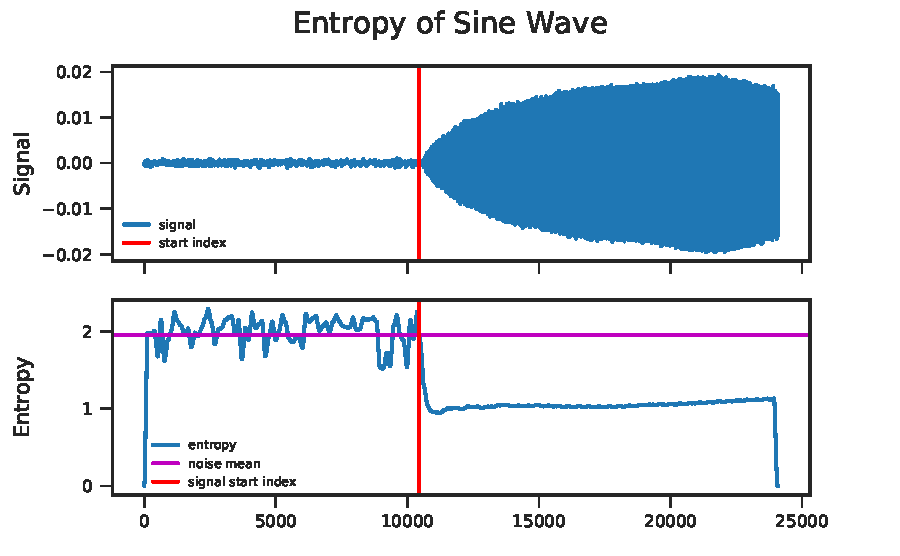
\includegraphics[]{figures/sine_entropy}
	\caption{Entropy of a sinusoidal signal with 3000Hz.}
\end{figure}
\label{fig:03_entropy}

\subsubsection*{Energy}

\ref{eq:02_energy} results in the energy of each frequency component of each frame.
According to this, the energy of one frame is \ref{eq:02_energy}
As the frames of the whole signal are overlapping, the energy function plotted in
\ref{fig:03_energy} results from overlapping and adding the frame energies.\\
- with a priori knowledge: only look for energy between 2000Hz and 4000Hz
One downside of the energy information is that the threshold can not be
set dynamically. It has to be adapted manually for the related environment.

\begin{figure}[ht]
	\centering
		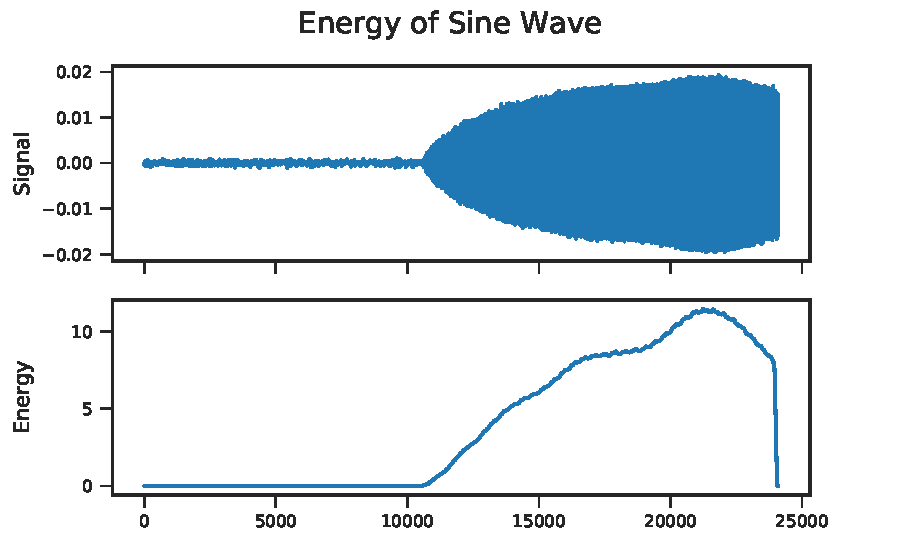
\includegraphics[]{figures/sine_energy}
	\caption{Energy of a sinusoidal signal with 3000Hz.}
\end{figure}
\label{fig:03_energy}

\code{signal_processing}{7}{19}{Whistle energy}

\subsubsection*{Zero Crossing Rate}

- count the sign changes in frame
- calculate the noise mean at the beginning of signal
- calculate signal mean at end of signal
- mean of both is set as threshold
- start index is detected at that point where zcr is higher than this threshold

\begin{figure}[ht]
	\centering
		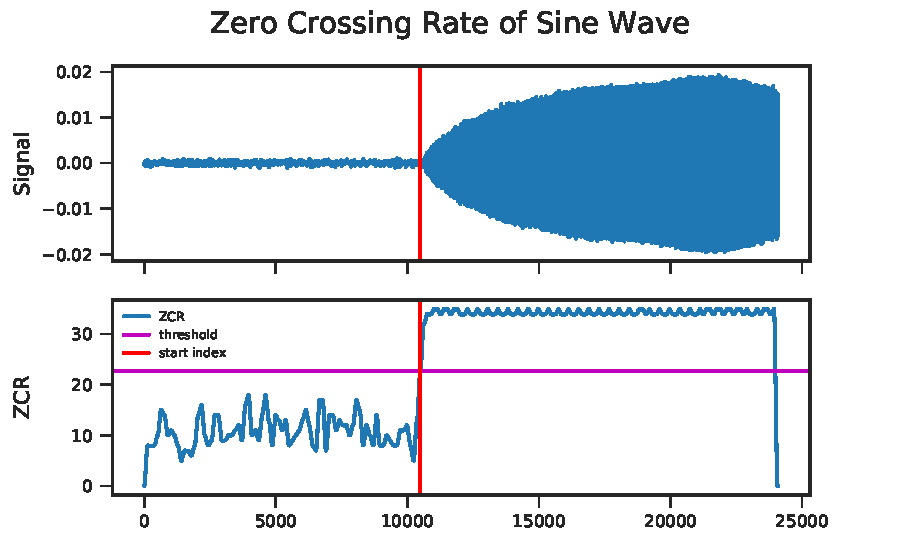
\includegraphics[]{figures/sine_zcr}
	\caption{Zero Crossing Rate of a sinusoidal signal with 3000Hz.}
\end{figure}
\label{fig:03_zcr}